\documentclass[noinstructornotes]{ximera}
%handout:  for handout version with no solutions or instructor notes
%handout,instructornotes:  for instructor version with just problems and notes, no solutions
%noinstructornotes:  shows only problem and solutions

%% handout
%% space
%% newpage
%% numbers
%% nooutcomes

%I added the commands here so that I would't have to keep looking them up
%\newcommand{\RR}{\mathbb R}
%\renewcommand{\d}{\,d}
%\newcommand{\dd}[2][]{\frac{d #1}{d #2}}
%\renewcommand{\l}{\ell}
%\newcommand{\ddx}{\frac{d}{dx}}
%\everymath{\displaystyle}
%\newcommand{\dfn}{\textbf}
%\newcommand{\eval}[1]{\bigg[ #1 \bigg]}

%\begin{image}
%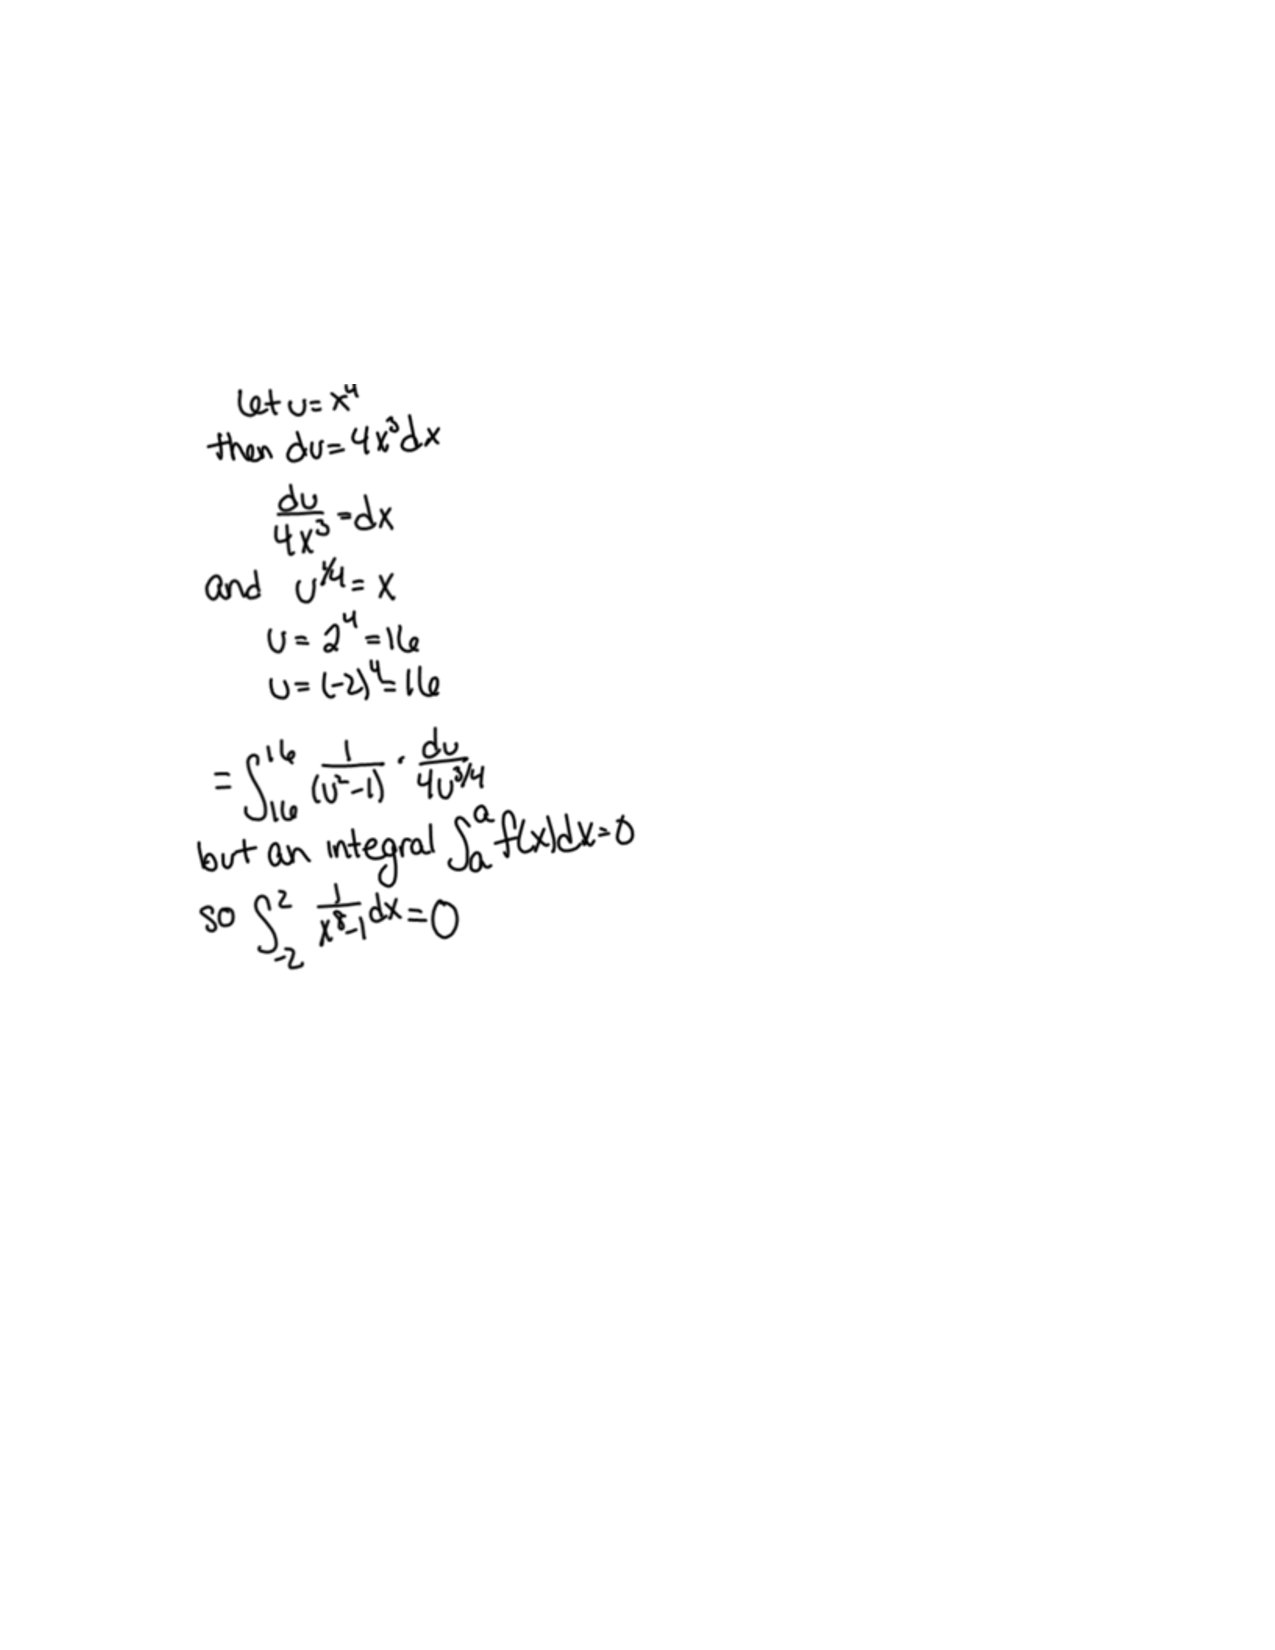
\includegraphics[trim= 170 420 250 180]{Figure1.pdf}
%\end{image}

%add a ``.'' below when used in a specific directory.
\newcommand{\RR}{\mathbb R}
\renewcommand{\d}{\,d}
\newcommand{\dd}[2][]{\frac{d #1}{d #2}}
\renewcommand{\l}{\ell}
\newcommand{\ddx}{\frac{d}{dx}}
\newcommand{\dfn}{\textbf}
\newcommand{\eval}[1]{\bigg[ #1 \bigg]}

\usepackage{multicol}

\renewenvironment{freeResponse}{
\ifhandout\setbox0\vbox\bgroup\else
\begin{trivlist}\item[\hskip \labelsep\bfseries Solution:\hspace{2ex}]
\fi}
{\ifhandout\egroup\else
\end{trivlist}
\fi} %% we can turn off input when making a master document

\title{Section 7.5: Partial Fractions}  

\begin{document}
\begin{abstract}		\end{abstract}
\maketitle



\section{Warm up:}
\begin{problem}
Give the general partial fraction decomposition for the following function.  DO NOT SOLVE FOR THE CONSTANTS! $$f(x) = \dfrac{4x^3-7}{x^6-x^2}$$

\end{problem}	


\section{Group work:}



%problem 1
\begin{problem}
Without determining the coefficients, write the partial fraction decomposition of the following rational function:
	\[
	\frac{5x^{13} - 6x^{12} + 7x^3 - 5x - 18}{(2x-3)(5x+9)^3 (x^2+9x+19)(x^2+9x+21)^2}
	\]
		
\end{problem}



%problem 2
\begin{problem}
Evaluate:
	\[
	\int \frac{7x^3 + 18x + 9}{x^4 + 9x^2} \d x
	\]
{\it Hint:  If $f(x) = 7x^3 + 18x + 9$, then $f(2) = 101$, $f(1) = 34$, and $f(-1) = -16$.}
	
		
\end{problem}















	
	
	
	
	
	
	
	
	

	










								
				
				
	














\end{document} 


















